\documentclass[10pt,a4paper]{article}
\usepackage[T1]{fontenc}
\usepackage[utf8]{inputenc}
\usepackage{lmodern}
\usepackage[margin=20mm]{geometry}
\usepackage{amsmath,amssymb,array,longtable,booktabs,calc,enumitem}
\usepackage{xurl,xcolor,mdframed}
\usepackage{float}
\usepackage{graphicx}
\usepackage[unicode,hidelinks]{hyperref}
\setlength{\parindent}{0pt}\setlength{\parskip}{5pt}
\setlength{\emergencystretch}{3em}\setlength{\tabcolsep}{4pt}
\renewcommand{\arraystretch}{1.12}\allowdisplaybreaks
\newcolumntype{L}[1]{>{\raggedright\arraybackslash}p{#1}}
\DeclareMathOperator{\CVaR}{CVaR}
\DeclareMathOperator{\logit}{logit}
\begin{document}

%%%%%%%%%%

\section{Two-stage ER-DRO model (CVaR-type ambiguity set)}

Data: $(x^k,p^k)$, $k=1,\dots,N$; for example, the context $x^k$ (zero-vehicle household share) and the robotaxi choice probability $p^k$ observed per city--period in which robotaxis have operated. A regression yields $\hat f$ and the logit-scale residuals $\hat\varepsilon^k=\logit(p^k)-(\hat\beta_0+\hat\beta_1x^k)$ (\S\ref{sec:demand}); attaching one residual at a time to the context $x_c$ of candidate city $c$ generates the scenarios $D_c^s$. Since one residual corresponds to one scenario, the scenario set $S$ is the index set of the residuals and $|S|=N$.
Below, the model is written as the first-stage problem (1), the per-scenario second-stage problem (3), and the extensive form \eqref{eq:ext} that is actually solved. The first-stage variables are $(y,q)$, and the second-stage variables $(O^s,U^s)$ are separable by scenario $s$.
No separate term is kept for the per-vehicle deployment/operating cost. Since every term of the model is expressed in trip units, the per-vehicle cost $K_c$ is converted into a cost per unit of capacity $K_c/\kappa_c$ and absorbed into $c_c^+$, $c_c^-$ (\S\ref{sec:absorb}); keeping it as an independent term does not change the optimal solution.

\subsection{First-stage problem}

\begin{subequations}\label{eq:first}
\begin{align}
\min_{y,q}\quad
 & \underbrace{\sum_{c\in C}F_c y_c}_{\text{entry cost}}
 + \underbrace{\mathcal R_\zeta(q)}_{\text{CVaR of scenario penalties}} \label{eq:1a}\\
\text{s.t.}\quad
 & 0\le q_c\le \bar q_c\,y_c, && \forall c\in C, \label{eq:1b}\\
 & \sum_{c\in C} q_c\le Q, \label{eq:1c}\\
 & y_c\in\{0,1\},\ q_c\in\mathbb Z_{\ge 0}, && \forall c\in C. \label{eq:1d}
\end{align}
\end{subequations}
Here $\mathcal R_\zeta(q)$ is the CVaR of the second-stage cost $H(q,D^s)$ over the scenario distribution, written in the Rockafellar--Uryasev threshold form
\begin{equation}\label{eq:cvar}
\mathcal R_\zeta(q)=\min_{\tau\in\mathbb R}\Big\{\tau+\frac{1}{|S|(1-\zeta)}\sum_{s\in S}\big(H(q,D^s)-\tau\big)^+\Big\}.
\end{equation}
When $\zeta=0$, $\mathcal R_0(q)=\frac1{|S|}\sum_s H(q,D^s)$ and the model reduces to ER-SAA (sample average). The context $x_c$ enters only through the scenario values $D_c^s=M_c p_c^s$; the optimization structure is unchanged.

\subsection{Second-stage problem (per-scenario recourse)}

Given the first-stage decision $q$ and the demand $D^s=(D_c^s)_{c\in C}$ of scenario $s$, the second-stage cost is
\begin{subequations}\label{eq:second}
\begin{align}
H(q,D^s)=\min_{O^s,U^s}\quad
 & \sum_{c\in C}\big(c_c^+O_c^s+c_c^-U_c^s\big) \label{eq:3a}\\
\text{s.t.}\quad
 & \kappa_c q_c-D_c^s=O_c^s-U_c^s, && \forall c\in C, \label{eq:3b}\\
 & O_c^s,\ U_c^s\ge 0, && \forall c\in C. \label{eq:3c}
\end{align}
\end{subequations}
(3) is also separable by $c$, and its optimal solution has the closed form $O_c^s=(\kappa_c q_c-D_c^s)^+$, $U_c^s=(D_c^s-\kappa_c q_c)^+$. Hence $H(q,D^s)=\sum_c\big[c_c^+(\kappa_c q_c-D_c^s)^+ + c_c^-(D_c^s-\kappa_c q_c)^+\big]$ is a convex piecewise-linear function of $q$, which is the basis for applying two-stage decomposition (L-shaped).
This second-stage cost has the same structure as the overage/underage cost of the newsvendor problem, and the first-stage decision $q$ is linked to the second stage only through the CVaR in (2).

\subsection{Demand model: $D_c^s=M_c\,p_c^s$ and the estimation of $p$}\label{sec:demand}

The robotaxi demand of city $c$ is the product $D_c=M_c\,p_c$ of the potential trip opportunities $M_c$ and the choice probability $p_c$, and uncertainty is placed only in $p_c$. $M_c$ is a fixed input, and $p_c$ is estimated by a logit model, i.e. a function of the exogenous context $x_c$ (ACS zero-vehicle household share) plus an error term.
\begin{equation}\label{eq:plogit}
\logit(p)=\ln\frac{p}{1-p}=\beta_0+\beta_1x+\varepsilon,\qquad
p=\sigma(\beta_0+\beta_1x+\varepsilon),\quad \sigma(z)=\frac{1}{1+e^{-z}},\quad \mathbb E[\varepsilon]=0 .
\end{equation}
Using observations $(x^k,p^k)$, $k=1,\dots,N$ from places where robotaxis have operated, $z^k=\logit(p^k)$ is fitted on $x^k$ by least squares to obtain $\hat\beta_0,\hat\beta_1$ and the residuals $\hat\varepsilon^k=z^k-\hat\beta_0-\hat\beta_1x^k$; for candidate city $c$ the residuals are attached one at a time to form scenarios.
\begin{equation}\label{eq:pscen}
p_c^{\,s}=\sigma\big(\hat\beta_0+\hat\beta_1x_c+\hat\varepsilon^{s}\big),\qquad D_c^{\,s}=M_c\,p_c^{\,s},\qquad s=1,\dots,N.
\end{equation}
Since $x_c$ is an exogenous variable independent of the decision $(y_c,q_c)$, all $D_c^s$ are constants computed before optimization, and the structure of \eqref{eq:first}--\eqref{eq:ext} is unchanged. The share $p$ rather than the demand $D$ is regressed because an error on the $D$ scale is proportional to $M_c$ and therefore heteroscedastic across city sizes, so the residuals could not be pooled into one sample.

There are two reasons for the logit form. First, $p$ is ``the probability that one trip opportunity chooses a robotaxi'', so the standard way to write a choice probability as a function of explanatory variables is the discrete-choice logit, which automatically guarantees $p\in(0,1)$ and monotonicity in $x$. Second, Loa et al.\ (2026), the only study analyzing observed robotaxi demand, report the zero-vehicle household share as a positive and significant variable in a log-linear spatial lag model with $\ln(\text{trips}+1)$ as the dependent variable; with $D=Mp$, a log-linear trip model has the same form as $\logit(p)\approx\ln p$ when $p$ is small, so \eqref{eq:plogit} is consistent with that result. This is also the basis for using a single context, the zero-vehicle household share.


\subsection{Extensive form: the MILP actually solved}

Linearizing $(\cdot)^+$ in (2) with variables $w^s$ and merging (3) into (1) gives the following single MILP. \eqref{eq:4b}--\eqref{eq:4c}, \eqref{eq:4g}--\eqref{eq:4h} are second-stage constraints separable by scenario, and \eqref{eq:4d}--\eqref{eq:4f} are first-stage constraints.
\begin{subequations}\label{eq:ext}
\begin{align}
\min_{y,q,O,U,\tau,w}\quad
 & \sum_{c\in C}F_c y_c+\tau+\frac{1}{|S|(1-\zeta)}\sum_{s\in S}w^s \label{eq:4a}\\
\text{s.t.}\quad
 & w^s\ge\sum_{c\in C}\big(c_c^+O_c^s+c_c^-U_c^s\big)-\tau, && \forall s\in S, \label{eq:4b}\\
 & \kappa_c q_c-D_c^s=O_c^s-U_c^s, && \forall c\in C,\ s\in S, \label{eq:4c}\\
 & 0\le q_c\le\bar q_c\,y_c, && \forall c\in C, \label{eq:4d}\\
 & \sum_{c\in C}q_c\le Q, \label{eq:4e}\\
 & y_c\in\{0,1\},\ q_c\in\mathbb Z_{\ge0}, && \forall c\in C, \label{eq:4f}\\
 & O_c^s,\ U_c^s\ge 0, && \forall c\in C,\ s\in S, \label{eq:4g}\\
 & w^s\ge 0,\ \ \tau\in\mathbb R, && \forall s\in S. \label{eq:4h}
\end{align}
\end{subequations}

\subsection{Variant: entry cost as a budget constraint}

If the number of cities that can be entered (or the entry budget) is the real constraint, remove $\sum_c F_c y_c$ from the objective \eqref{eq:4a} and add the following constraint.
\begin{equation}\label{eq:budget}
\sum_{c\in C}F_c y_c\le B \qquad\text{or}\qquad \sum_{c\in C}y_c\le B.
\end{equation}
In this variant only $\tau+\frac{1}{|S|(1-\zeta)}\sum_s w^s$, i.e. the CVaR of the second-stage penalty, remains in the objective. Because the variant directly restricts the combinations of $y$, it mitigates the problem in two-stage decomposition that the initial master problem returns the trivial solution ($y=q=0$) and the iterations become long.

\subsection{Absorption of the per-vehicle cost: why the $K_c$ term is dropped}\label{sec:absorb}

Even if the per-vehicle cost $K_c$ (deployment/operation) is placed in the objective as $\sum_c K_c q_c$, by \eqref{eq:4c} we have $\kappa_c q_c=D_c^s+O_c^s-U_c^s$ for every $s$, so for $\zeta=0$
\begin{equation}\label{eq:absorb}
\sum_{c}K_c q_c+\frac1{|S|}\sum_{s}\sum_{c}\big(c_c^+O_c^s+c_c^-U_c^s\big)
=\underbrace{\frac1{|S|}\sum_s\sum_c\frac{K_c}{\kappa_c}D_c^s}_{\text{constant independent of the decision}}
+\frac1{|S|}\sum_{s}\sum_{c}\Big[\Big(c_c^++\frac{K_c}{\kappa_c}\Big)O_c^s+\Big(c_c^--\frac{K_c}{\kappa_c}\Big)U_c^s\Big]
\end{equation}
holds. That is, $K_c$ is equivalent to the redefinition $c_c^+\leftarrow c_c^++K_c/\kappa_c$, $c_c^-\leftarrow c_c^--K_c/\kappa_c$ (for $\zeta>0$ the term $(K_c/\kappa_c)D_c^s$ enters the CVaR, so this is an approximation), and it is not an independent decision lever. Moreover, if $K_c$ is the same across cities and \eqref{eq:4e} binds with equality, $\sum_c K_c q_c=KQ$ is a constant. Therefore this study does not keep $K_c$ as a separate term; the per-vehicle cost converted to a per-trip-of-capacity value is regarded as included in the definitions of $c_c^+$, $c_c^-$, and only their ratio is considered (e.g. 1:5).

{\footnotesize
\begin{longtable}{@{}L{0.34\textwidth}L{0.12\textwidth}L{0.50\textwidth}@{}}
\toprule Constraint & Stage & Meaning\\\midrule\endhead\bottomrule\endlastfoot
$0\le q_c\le\bar q_c y_c$ \eqref{eq:4d} & stage 1 & no vehicles unless the city is entered; if entered, up to the per-city cap\\
$\sum_c q_c\le Q$ \eqref{eq:4e} & stage 1 & limit on the total number of vehicles\\
$\sum_c F_c y_c\le B$ \eqref{eq:budget} & stage 1 (variant) & limit on the entry budget (or number of entered cities); replaces $\sum_c F_c y_c$ in the objective\\
$\kappa_c q_c-D_c^s=O_c^s-U_c^s$ \eqref{eq:4c} & stage 2 (separable by $s$) & service capacity minus robotaxi demand $=$ surplus capacity $-$ unmet demand\\
$w^s\ge\sum_c(c_c^+O_c^s+c_c^-U_c^s)-\tau$, $w^s\ge0$ \eqref{eq:4b},\eqref{eq:4h} & stage 2 (separable by $s$) & amount by which the penalty of scenario $s$ exceeds the threshold $\tau$; in the minimization $w^s=(\text{penalty}_s-\tau)^+$\\
\end{longtable}}

\section{Notation}
\subsection{Additional notation for the contextual and DRO parts}
{\footnotesize
\begin{longtable}{@{}L{0.14\textwidth}L{0.45\textwidth}L{0.35\textwidth}@{}}
\toprule Symbol & Meaning & Type and unit\\\midrule\endhead\bottomrule\endlastfoot
$(x^k,p^k)$ & context (zero-vehicle household share) and robotaxi choice probability of observation $k$ & data; $k=1,\dots,N$\\
$x_c$ & covariate vector of candidate city $c$; at this stage a single variable, the zero-vehicle household share & input; corresponds to the new observation $x$ in Kannan et al.\\
$\hat f$ & estimated regression function; $\hat f(x)\approx\mathbb E[p\mid x]$. Logit $\hat f(x)=\sigma(\hat\beta_0+\hat\beta_1x)$, $\sigma(z)=1/(1+e^{-z})$ & estimated function\\
$\hat\varepsilon^k$ & residual $\logit(p^k)-(\hat\beta_0+\hat\beta_1x^k)$ & derived; logit scale\\
$\zeta$ & radius (tail fraction) of the CVaR-type ambiguity set; $1-\zeta$ is the fraction of scenarios kept as the worst group & input; $[0,1)$; $\zeta=0$ gives ER-SAA\\
$\tau$ & penalty threshold; a decision variable equal at the optimum to ``the $|S|(1-\zeta)$-th largest penalty'' & decision variable; monetary unit\\
$w^s$ & amount by which the penalty of scenario $s$ exceeds $\tau$ & decision variable; monetary unit\\
$\mathcal R_\zeta(q)$ & CVaR of the second-stage cost, eq.\ \eqref{eq:cvar} & function of $q$; monetary unit\\
$H(q,D^s)$ & second-stage (recourse) cost of scenario $s$, eq.\ \eqref{eq:second} & function of $q$; monetary unit\\
$B$ & entry budget or number of cities that can be entered (variant) & input; monetary unit or number of cities\\
\end{longtable}}

\subsection{Basic notation}
{\footnotesize
\begin{longtable}{@{}L{0.10\textwidth}L{0.43\textwidth}L{0.41\textwidth}@{}}
\toprule Symbol & Meaning & Type and unit\\\midrule\endfirsthead
\toprule Symbol & Meaning & Type and unit\\\midrule\endhead\bottomrule\endlastfoot
$C$ & set of candidate cities & input set; cities\\
$S$ & set of demand scenarios & input set; index set of residuals, $|S|=N$\\
$y_c$ & 1 if city $c$ is entered, 0 otherwise & first-stage decision; binary\\
$q_c$ & number of vehicles deployed in city $c$ & first-stage decision; vehicles (integer)\\
$\kappa_c$ & trips one vehicle can serve during the evaluation period & scale parameter; trips/vehicle\\
$Q$ & total number of vehicles available for deployment (owned fleet; acquisition cost and depreciation are sunk) & input; vehicles\\
$\bar q_c$ & per-city deployment cap & input; vehicles\\
$F_c$ & fixed cost of entry and basic infrastructure & input; monetary unit per evaluation period\\
$c_c^+$ & loss per unit of surplus capacity & input; money/trip\\
$c_c^-$ & opportunity loss per unit of unmet potential demand; eq.\ \eqref{eq:absorb} & input; money/trip\\
$M_c$ & annual number of \textbf{potential trip opportunities over all modes} in city $c$ & input; opportunities; data or assumption\\
$p_c^s$ & probability that a trip opportunity in city $c$ chooses a robotaxi & generated by regression; $[0,1]$; $p_c^s=\sigma(\hat\beta_0+\hat\beta_1x_c+\hat\varepsilon^s)$\\
$D_c^s$ & robotaxi demand & derived input; trips; $D_c^s=M_c p_c^s$\\
$O_c^s$ & surplus service capacity & second-stage outcome; trips; $O_c^s=(\kappa_c q_c-D_c^s)^+$\\
$U_c^s$ & unmet robotaxi demand & second-stage outcome; trips; $U_c^s=(D_c^s-\kappa_c q_c)^+$\\
\end{longtable}}


%%%%%%%%%%%%%%%%%%%%%%%%%%%%%%%%%%%%%%%%
\section{Numerical experiments: synthetic data}

\subsection{Overall flow}

In a synthetic environment where the true demand model is known, we measure (i) whether the estimation--optimization pipeline works, and (ii) quantities that can only be measured when the true model is available (out-of-sample cost, value of context, effect of DRO). The flow has five steps.
\begin{enumerate}[nosep]
  \item Set the candidate-city inputs $(x_c, M_c, \kappa_c, \bar q_c, F_c)$ and the true demand model $p=\sigma(\beta_0+\beta_1 x+\varepsilon)$.
  \item Generate training data $(x^k,p^k)_{k=1}^N$ from the true model and estimate $\hat f$ and the residuals $\hat\varepsilon^k$ by logit OLS.
  \item Build the per-city scenarios $D_c^s=M_c\,\sigma(\hat\beta_0+\hat\beta_1x_c+\hat\varepsilon^s)$ and solve the extensive form \eqref{eq:ext}.
  \item Compute the out-of-sample expected cost and tail cost of the solution $(y,q)$ on 1{,}000 evaluation scenarios generated separately from the true model.
  \item Repeat 2--4 over the settings $(N, c^-, \zeta)$ and compare with the no-context benchmark and the variant \eqref{eq:budget}.
\end{enumerate}

\subsection{Synthetic data generation}\label{sec:data}

\paragraph{Candidate-city inputs.}
The candidate cities are the 18 cities Waymo has announced as future expansion candidates. Each city is mapped to one central county (e.g. Chicago $\to$ Cook County), and the context $x_c$ is the actual zero-vehicle household share from ACS 2019--2023 5-year estimates, table B08201 (range $0.054$--$0.777$; New York County at 0.777 is an extreme value covering Manhattan only). The potential trip opportunities $M_c$ are the total households in the same ACS table multiplied by a proportionality constant of 10; this constant is a toy assumption (with real data it is replaced by the NHTS $\times$ ACS cross-classification). The remaining inputs are common to all cities (Table~\ref{tab:param}).

\paragraph{True demand model.}

The true model is the logit model \eqref{eq:plogit} of \S\ref{sec:demand} with $\varepsilon\sim N(0,\sigma_\varepsilon^2)$.
\begin{equation}\label{eq:truth}
\logit(p)= \beta_0+\beta_1 x+\varepsilon,\qquad \varepsilon\sim N(0,\sigma_\varepsilon^2).
\end{equation}
$\beta_1=0.8$ is the zero-vehicle household share coefficient $0.008$ per \%-point ($t=7.4$) in Table 3 of Loa et al.\ (2026) rescaled to the 0--1 scale ($0.008\times100$). $\beta_0=-3.5$ and $\sigma_\varepsilon=0.3$ are assumptions chosen so that $p$ falls roughly in the range $0.03$--$0.09$.

\paragraph{Base parameters.}
Costs are normalized with $c^+=1$ and $c^-$ is varied over $1, 5, 10$ (to examine the effect of the overage-to-underage cost ratio $c^+:c^-$ on the decision). The entry cost is set as $F_c=F_0\,c^-$ so that the ``entry cost to unmet margin'' ratio stays independent of $c^-$.

\begin{table}[H]\centering\small
\caption{Base parameters and rationale}\label{tab:param}
\begin{tabular}{@{}llp{0.55\textwidth}@{}}
\toprule
Parameter & Value & Rationale \\ \midrule
$x_c$ & actual ACS values (0.054--0.777) & ACS 2019--2023 B08201, county level \\
$M_c$ & total households $\times$ 10 & household counts are actual ACS values; the constant is a toy assumption \\
$\kappa_c$ & 8{,}760 trips/vehicle/year & 24 trips/day $\times$ 365 days (sensitivity 6570--10950); 24 trips per vehicle per day back-calculated from Waymo's public figures \\
$\bar q_c$ & 150 vehicles & assumption (sensitivity 50--300) \\
$Q$ & $0.6\times\mathbb E[\sum_c D_c]/\kappa$ & assumption; only 60\% of expected demand can be served, so that the allocation is non-trivial \\
$F_0$ & $10^5$ (at $c^-=1$) & assumption (sensitivity $0.25\times10^5$--$4\times10^5$) \\
$c^+:c^-$ & $1:1,\ 1:5,\ 1:10$ & assumption \\
$\beta_0,\beta_1,\sigma_\varepsilon$ & $-3.5,\ 0.8,\ 0.3$ & $\beta_1$ rescaled from Loa et al.; $\beta_0$, $\sigma_\varepsilon$ assumed \\
$N$ & 15, 200 & scarce/ample city--period observations; number of training observations $=$ number of scenarios $|S|$ \\
$\zeta$ & 0, 0.5, 0.9 & 0 = ER-SAA; 0.9 = default \\
Evaluation scenarios & 1{,}000 & arbitrary assumption \\
\bottomrule
\end{tabular}
\end{table}

\subsection{Training and evaluation data}

\paragraph{Training data.}
These mimic ``$(x,p)$ observed in city--periods where robotaxis have already operated''. Random $x^k$ are drawn uniformly over the range of the candidate-city $x_c$, $\varepsilon^k$ is drawn from the true model~\eqref{eq:truth}, and $p^k$ is computed ($k=1,\dots,N$). Without knowing the true coefficients, the model estimates $\hat\beta_0,\hat\beta_1$ and the residuals $\hat\varepsilon^k$ from these $N$ points, and the optimization sees only the scenarios built from those estimates. With real data this step is replaced by an observed table with $x$ = ACS share and $p$ = robotaxi trips$/M$.

\paragraph{Evaluation data.}
These mimic ``the demand that actually materializes after the decision is made''. The true coefficients are applied to the actual $x_c$ of the candidate cities, and 1{,}000 draws of $\varepsilon$ independent of the training data produce $D^{\mathrm{eval}}_{c}$ (18 candidate cities $\times$ 1{,}000). The optimization never sees these data; once $(y,q)$ is fixed, the per-scenario cost is computed in the closed form of eq.~\eqref{eq:second} and scored by the mean (expected cost) and the mean of the top 10\% (tail cost, $\CVaR_{0.9}$). Because the evaluation data are fixed independently of $N$, the decisions made with $N=15$ and $N=200$ are compared on the same yardstick. The value scored on the training data (in-sample) is optimistic because the optimization was fitted to those data, which is why in-sample and OOS differ in Table~\ref{tab:main}.

\paragraph{Solution method comparison: extensive form vs.\ L-shaped decomposition.}
The two-stage model \eqref{eq:first}--\eqref{eq:second} was solved (i) as a whole in the extensive form \eqref{eq:ext} and (ii) by multi-cut L-shaped decomposition into a master $(y,q,\tau)$ and per-scenario subproblems ($N=15$, $c^-=5$, $\zeta=0.9$; the decomposition stops at $\mathrm{UB}-\mathrm{LB}\le 10^{-2}\,|\mathrm{UB}|$, i.e. a 1\% relative tolerance).

\begin{table}[H]\centering\small
\caption{Extensive form vs.\ L-shaped decomposition}\label{tab:solver}
\begin{tabular}{@{}llrrl@{}}
\toprule
Setting & Method & Objective & Time & Note \\ \midrule
$B=3$ & extensive & 16{,}036{,}515 & 0.4 s & entered: Chicago, New York, San Diego \\
      & L-shaped & 16{,}140{,}861 & 29.5 s & 38 iterations, same cities, difference 0.65\% \\
no $B$ & extensive & 17{,}304{,}198 & 1.5 s & entered: Chicago, New York, Philadelphia, Seattle \\
      & L-shaped & 17{,}378{,}353 & 54.5 s & 38 iterations, difference 0.43\%, 2 cities differ \\
\bottomrule
\end{tabular}
\end{table}

The L-shaped objective was 0.65\% higher than the extensive form for $B=3$ and 0.43\% higher without $B$; the entered cities were identical for $B=3$ but two differed without $B$. Since the value returned by L-shaped is the cost of the feasible solution at termination (an upper bound), the difference is the result of stopping early at the tolerance, and it shows that without $B$ a different city combination is feasible at a cost 0.43\% higher. Computation times were 0.4 s and 1.5 s for the extensive form versus 29.5 s and 54.5 s for L-shaped, so the extensive form was far faster, because the second-stage cost is the max of two affine functions and the $O,U$ variables of the extensive form amount to including all cuts from the start. Moving the $F_c y_c$ term into the constraint $B$ ($\sum_{c\in C}y_c\le B$) reduces the convergence time of the decomposition. All subsequent experiments use the extensive form; the comparison will be revisited for the decision-dependent extension.

\subsection{Analysis of results}

The experimental setting is as in \S\ref{sec:data}, and the total fleet computed from the true model is $Q=267$ vehicles. Every solution is evaluated out of sample on 1{,}000 true-model scenarios (expected cost and tail cost = mean of the worst 10\%). The five questions below are each answered in the order answer, evidence, and the corresponding table/figure.

\paragraph{Summary.}
(Q1) Logit regression of $p$ recovers the true coefficients and satisfies the residual-pooling condition. (Q2) The conclusions are insensitive to the $c^+:c^-$ ratio, so $1:5$ is taken as the base. (Q3) Context reduces cost in proportion to how strongly $x$ drives demand (1--3\% in the current setting, 25--41\% with strong context); DRO gives up expected cost to reduce tail cost, and the two should be used together. (Q4) Even with 15 observations the cost stays within 3\%. (Q5) Cost is sensitive to the scale of $Q$, $\kappa$, $F_0$, $\sigma_\varepsilon$; Chicago and New York are selected in every setting and San Diego in 17 of 18.

%---------------------------------------
\paragraph{Q1. Can demand be estimated by a logit regression of $p$?}
In Table~\ref{tab:fit}, with $N=200$, $\hat\beta_1=0.67$ and $\hat\sigma_\varepsilon=0.30$ recover values close to the truth ($0.8$, $0.3$). The condition for pooling the residuals as scenarios (mean 0 and constant variance regardless of $x$) is confirmed by the residual scatter in Figure~\ref{fig:diag}. The low test $R^2$ of $0.12$--$0.14$ arises because, by construction, $x$ explains only about 13\% of the demand variation; using only the mean without $x$ gives $R^2\approx0$, so the explanatory power of $x$ is small but clearly present.

\begin{table}[H]\centering\small
\caption{Logit OLS estimates (error metrics on the $p$ scale, 1{,}000 test observations)}\label{tab:fit}
\begin{tabular}{@{}rrrrrrrrr@{}}
\toprule
$N$ & $\hat\beta_0$ & $\hat\beta_1$ & $\hat\sigma_\varepsilon$ & test MSE & test MAE & test ME & test $R^2$ & no-context $R^2$ \\ \midrule
15  & $-3.655$ & $1.114$ & $0.325$ & $0.0002$ & $0.0101$ & $0.0461$ & $0.124$ & $-0.011$ \\
200 & $-3.479$ & $0.665$ & $0.298$ & $0.0002$ & $0.0099$ & $0.0479$ & $0.143$ & $-0.013$ \\
true & $-3.500$ & $0.800$ & $0.300$ & & & & & \\
\bottomrule
\end{tabular}
\end{table}

\begin{figure}[H]\centering
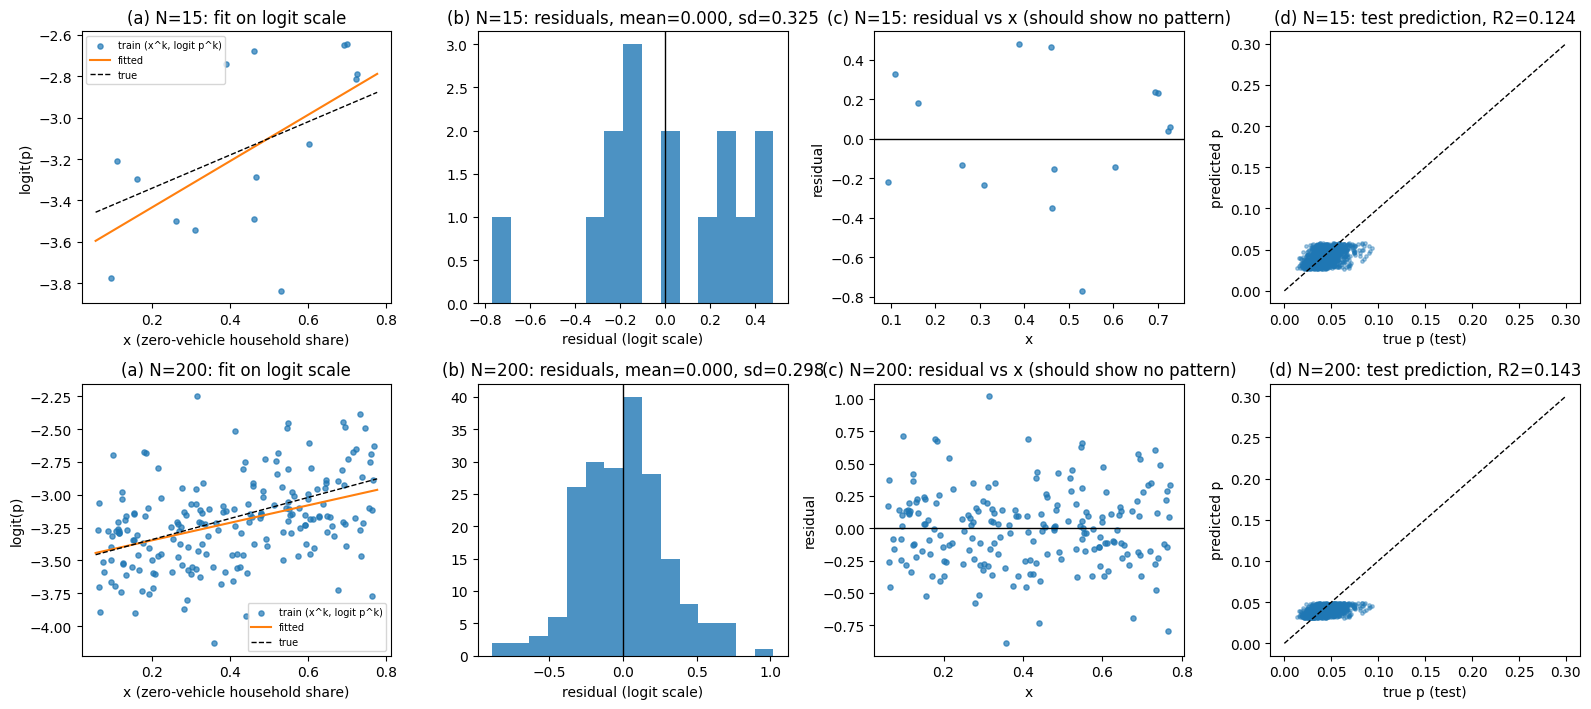
\includegraphics[width=\textwidth]{figures/fig1_f_diagnostics.png}
\caption{Diagnostics of the estimate of $f$. (a) data, fitted line and true line on the logit scale, (b) residual distribution, (c) residual vs.\ $x$, (d) predicted vs.\ true $p$ on the test data. Top row $N=15$, bottom row $N=200$.}\label{fig:diag}
\end{figure}

%---------------------------------------------------------------
\paragraph{Q2. Which $c^+:c^-$ ratio should be used?}
The ratio is an input chosen in the absence of data, and the role of the experiment is to show that the conclusions do not change with it. In Table~\ref{tab:main}, for all of $c^-=1,5,10$: (i) the context model has lower OOS expected cost than the no-context model, (ii) the number of entered cities falls as $\zeta$ grows, and (iii) Chicago and New York are selected in all 18 settings and San Diego in 17. In the $c^-$ panel of Figure~\ref{fig:sens}, cost grows in proportion to $c^-$ (3.08, 5.79, 14.22, 27.63, 54.45M at $c^-=1,2,5,10,20$) but the relative order of the three models does not change. Therefore the base setting is $1:5$, where underage is costlier than overage, and the other ratios are only reported.

\begin{table}[H]\centering\footnotesize
\caption{Optimal number of entered cities, in-sample objective, OOS cost ($c^+=1$ units) and context gain by setting}\label{tab:main}
\begin{tabular}{@{}rrr r rrr rr r@{}}
\toprule
$N$ & $c^-$ & $\zeta$ & \# entered & in-sample & OOS mean & OOS tail & no-ctx mean & no-ctx tail & gain \\ \midrule
15  & 1  & 0   & 9 & 2{,}490{,}926 & 2{,}695{,}476 & 4{,}857{,}473 & 2{,}758{,}361 & 4{,}657{,}473 & 2\% \\
    &    & 0.5 & 6 & 2{,}864{,}469 & 2{,}724{,}601 & 4{,}557{,}473 & 3{,}112{,}997 & 4{,}357{,}473 & 12\% \\
    &    & 0.9 & 4 & 3{,}460{,}840 & 3{,}147{,}884 & 4{,}410{,}069 & 3{,}869{,}252 & 4{,}739{,}552 & 19\% \\
    & 5  & 0   & 6 & 11{,}386{,}313 & 12{,}541{,}832 & 22{,}787{,}364 & 12{,}702{,}986 & 22{,}787{,}364 & 1\% \\
    &    & 0.5 & 5 & 13{,}635{,}159 & 12{,}712{,}913 & 22{,}287{,}364 & 14{,}896{,}198 & 22{,}208{,}291 & 15\% \\
    &    & 0.9 & 4 & 17{,}304{,}198 & 13{,}787{,}444 & 21{,}975{,}797 & 15{,}636{,}705 & 23{,}199{,}859 & 12\% \\
    & 10 & 0   & 6 & 22{,}412{,}124 & 24{,}728{,}335 & 45{,}574{,}729 & 25{,}166{,}440 & 45{,}574{,}729 & 2\% \\
    &    & 0.5 & 5 & 27{,}186{,}803 & 25{,}027{,}407 & 44{,}574{,}729 & 28{,}863{,}429 & 44{,}263{,}095 & 13\% \\
    &    & 0.9 & 4 & 34{,}608{,}397 & 27{,}416{,}340 & 43{,}920{,}442 & 30{,}089{,}296 & 45{,}739{,}579 & 9\% \\ \midrule
200 & 1  & 0   & 8 & 2{,}599{,}840 & 2{,}662{,}764 & 4{,}757{,}473 & 2{,}748{,}503 & 4{,}657{,}473 & 3\% \\
    &    & 0.5 & 6 & 3{,}054{,}078 & 2{,}712{,}652 & 4{,}557{,}473 & 2{,}980{,}460 & 4{,}457{,}473 & 9\% \\
    &    & 0.9 & 4 & 4{,}415{,}710 & 3{,}084{,}216 & 4{,}357{,}473 & 3{,}727{,}040 & 4{,}610{,}719 & 17\% \\
    & 5  & 0   & 6 & 12{,}225{,}772 & 12{,}463{,}377 & 22{,}787{,}364 & 12{,}722{,}661 & 22{,}787{,}364 & 2\% \\
    &    & 0.5 & 5 & 14{,}870{,}099 & 12{,}674{,}534 & 22{,}287{,}364 & 13{,}031{,}319 & 22{,}287{,}364 & 3\% \\
    &    & 0.9 & 3 & 22{,}045{,}780 & 14{,}222{,}971 & 21{,}617{,}923 & 14{,}901{,}907 & 22{,}265{,}378 & 5\% \\
    & 10 & 0   & 6 & 24{,}168{,}288 & 24{,}654{,}132 & 45{,}574{,}729 & 25{,}128{,}612 & 45{,}574{,}729 & 2\% \\
    &    & 0.5 & 5 & 29{,}646{,}948 & 24{,}957{,}044 & 44{,}574{,}729 & 25{,}611{,}150 & 44{,}574{,}729 & 3\% \\
    &    & 0.9 & 3 & 44{,}013{,}689 & 27{,}629{,}179 & 43{,}180{,}752 & 28{,}889{,}111 & 44{,}519{,}917 & 4\% \\
\bottomrule
\end{tabular}
\end{table}

%---------------------------------------------------------------
\paragraph{Q3. Why contextual ER-DRO, and are its conditions satisfied?}
The conditions were confirmed in Q1 (independence of the residuals from $x$ and consistency of $\hat f$). The effect has two parts. \emph{Effect of context}: in Table~\ref{tab:main}, the OOS expected-cost gain of the context model is 1--3\% at $\zeta=0$, 3--15\% at $\zeta=0.5$ and 4--19\% at $\zeta=0.9$. The gain is small because $x$ has little explanatory power at $\beta_1=0.8$; in the $\beta_1$ panel of Figure~\ref{fig:sens}, the two models have equal cost at $\beta_1=0$, and the gain grows to 1\%, 16\%, 25\%, 41\% at $\beta_1=0.8, 1.5, 3, 5$. \emph{Effect of DRO}: $\zeta$ trades expected cost against tail cost. For $N=200$, $c^-=5$, as $\zeta=0\to0.5\to0.9$ the expected cost is $12.46\to12.67\to14.22$M ($+1.7\%$, $+14\%$) and the tail cost is $22.79\to22.29\to21.62$M ($-2.2\%$, $-5.1\%$) (Figure~\ref{fig:zeta}). Meanwhile, the no-context model at $N=15$, $\zeta=0.9$ has a tail cost that is actually higher than at $\zeta=0$ ($c^-=5$: 22.79M$\to$23.20M; likewise for $c^-=1,10$). This arises from trying to fit the tail with only 15 residuals and no $x$, and it means DRO should be used together with context.

\begin{figure}[H]\centering
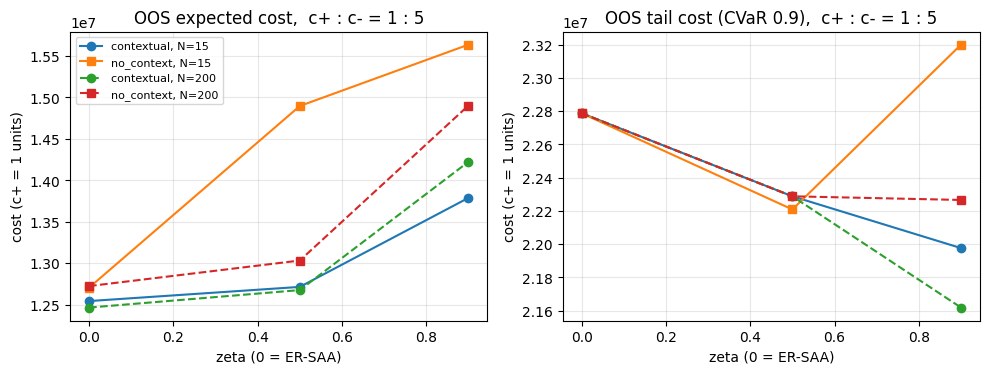
\includegraphics[width=0.9\textwidth]{figures/toy_oos_vs_zeta.png}
\caption{OOS expected cost (left) and tail cost (right) vs.\ $\zeta$, $c^+:c^-=1:5$.}\label{fig:zeta}
\end{figure}

%---------------------------------------------------------------
\paragraph{Q4. Can the model be used with scarce data?}
Yes, if context is used. In the $\zeta=0.9$ rows of Table~\ref{tab:main}, the OOS expected-cost difference between $N=15$ and $N=200$ is 2.1\%, 3.1\%, 0.8\% for $c^-=1,5,10$, and the tail-cost difference is 1.2--1.7\%. This holds even though $\hat\beta_1$ is overestimated by 39\% at $N=15$ and only the top 2 scenarios enter the objective at $\zeta=0.9$. In the $N$ panel of Figure~\ref{fig:sens}, ER-SAA (context) is flat within 1.4\% from $N=10$ to $200$, while ER-DRO (context) fluctuates over 13.19--14.24M and the no-context model over 14.38--16.14M. That is, the advantage of the context model grows as data become scarcer.

%---------------------------------------------------------------
\paragraph{Q5. Sensitivity.}
Figure~\ref{fig:sens} changes one parameter at a time from the base setting ($N=200$, $c^-=5$, $\zeta=0.9$). Cost rises with the entry cost $F_0$ and the variability $\sigma_\varepsilon$ ($F_0$: 12.04$\to$18.73M) and falls with the total fleet $Q$ and the per-vehicle throughput $\kappa$ ($Q$ ratio 0.2$\to$1.0: 16.79$\to$11.45M). When $Q$ is as small as 20\% of expected demand the three models have almost the same cost, because every vehicle is used however it is allocated. The per-city cap $\bar q_c$ does not change the result above 100 for ER-SAA and above 150 for ER-DRO. In the variant \eqref{eq:budget} of Table~\ref{tab:budget}, the second-stage cost falls as the number of entered cities grows over $B=2,3,5$ ($N=200$, $c^-=5$: 14.57$\to$12.73$\to$11.74M), and the first three cities are stable regardless of $N$ and $c^-$: Chicago, New York $\to$ San Diego. The composition at $B=5$ depends on $N$; at $N=200$, $c^-=5,10$, Philadelphia, Pittsburgh and Tampa enter instead of New York.

\begin{figure}[H]\centering
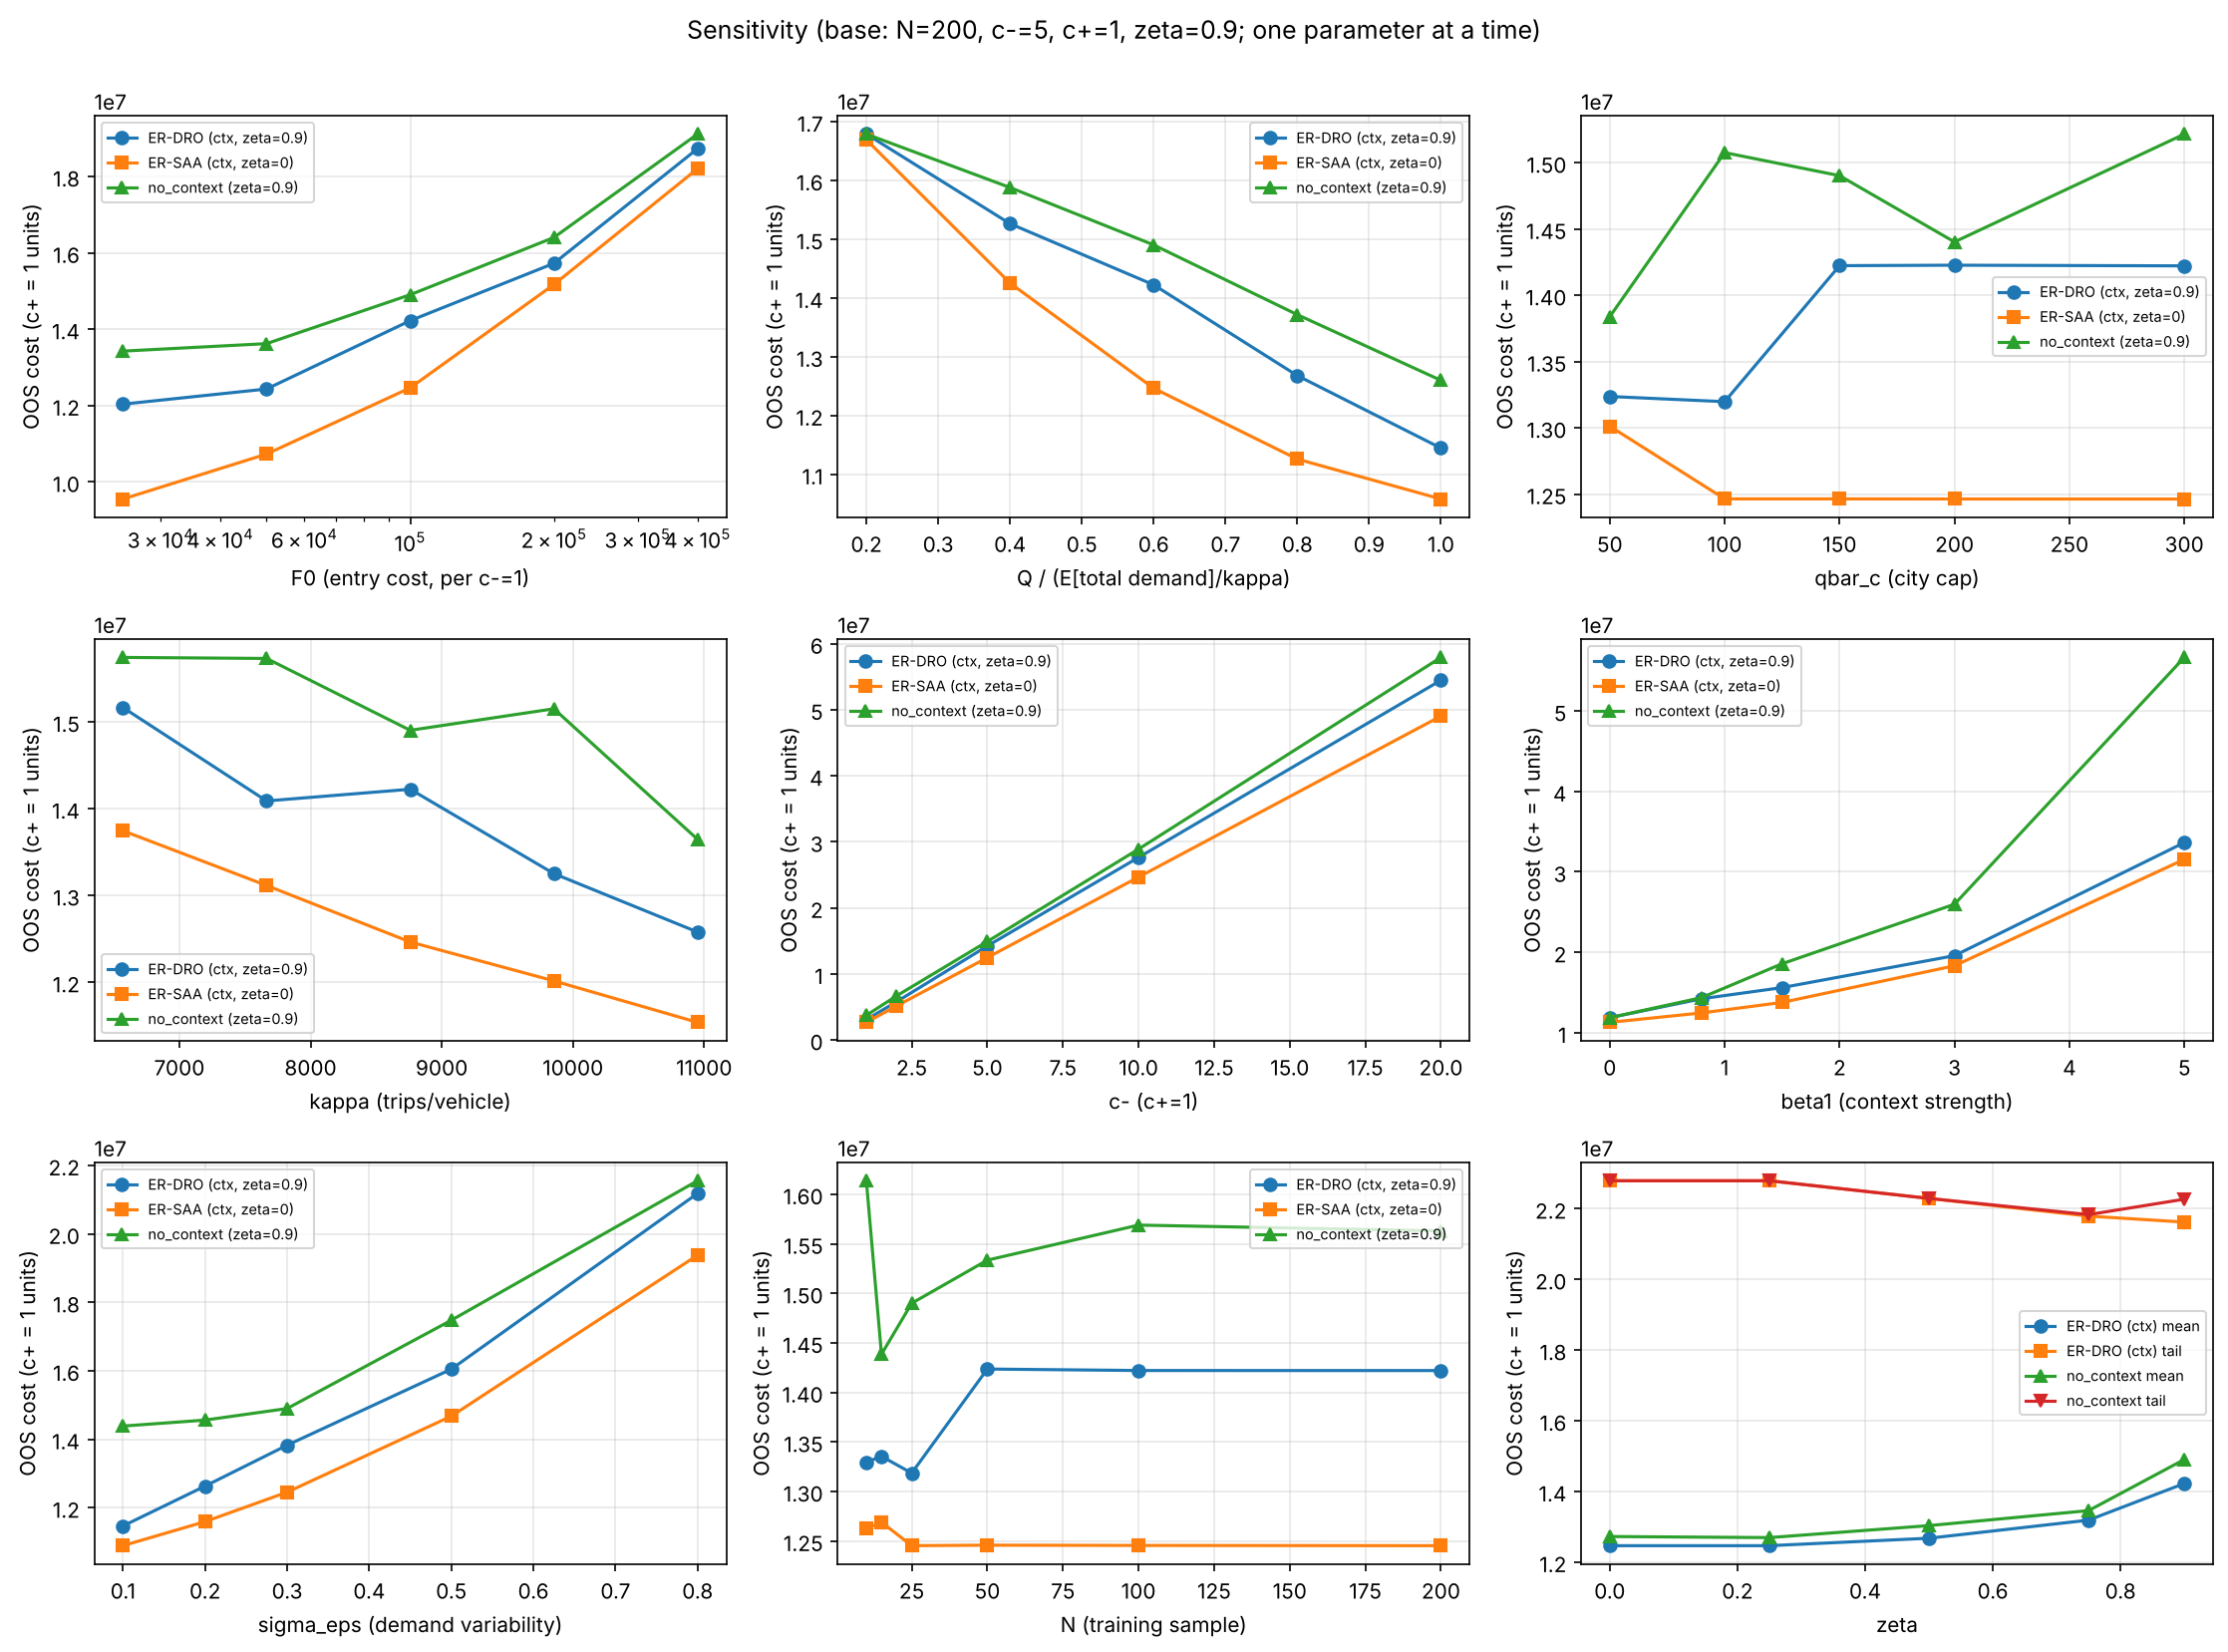
\includegraphics[width=\textwidth]{figures/fig2_sensitivity.png}
\caption{Sensitivity analysis. One parameter at a time from the base $N=200$, $c^-=5$, $c^+=1$, $\zeta=0.9$. Lines: context ER-DRO ($\zeta=0.9$), context ER-SAA ($\zeta=0$), no context ($\zeta=0.9$).}\label{fig:sens}
\end{figure}

\begin{table}[H]\centering\small
\caption{Variant \eqref{eq:budget}: OOS second-stage cost and selected cities by number of entered cities $B$ ($\zeta=0.9$)}\label{tab:budget}
\begin{tabular}{@{}rrrrl@{}}
\toprule
$N$ & $c^-$ & $B$ & OOS second-stage cost & Entered cities \\ \midrule
15  & 1  & 2 & 3{,}315{,}579 & Chicago, New York \\
    &    & 3 & 3{,}084{,}918 & + San Diego \\
    &    & 5 & 2{,}358{,}358 & + Philadelphia, Seattle \\
    & 5  & 2 & 14{,}339{,}887 & Chicago, New York \\
    &    & 3 & 12{,}668{,}561 & + San Diego \\
    &    & 5 & 10{,}305{,}798 & + Philadelphia, Seattle \\
    & 10 & 2 & 28{,}111{,}826 & Chicago, New York \\
    &    & 3 & 24{,}631{,}627 & + San Diego \\
    &    & 5 & 20{,}068{,}402 & + Philadelphia, Seattle \\ \midrule
200 & 1  & 2 & 3{,}395{,}462 & Chicago, New York \\
    &    & 3 & 3{,}198{,}004 & + San Diego \\
    &    & 5 & 2{,}440{,}092 & + Detroit, Philadelphia \\
    & 5  & 2 & 14{,}572{,}482 & Chicago, New York \\
    &    & 3 & 12{,}726{,}413 & + San Diego \\
    &    & 5 & 11{,}735{,}447 & Chicago, Philadelphia, Pittsburgh, San Diego, Tampa \\
    & 10 & 2 & 28{,}274{,}685 & Chicago, New York \\
    &    & 3 & 24{,}625{,}772 & + San Diego \\
    &    & 5 & 22{,}821{,}183 & Chicago, Philadelphia, Pittsburgh, San Diego, Tampa \\
\bottomrule
\end{tabular}
\end{table}

\clearpage

\section{\textcolor{red}{Plan for real-data application (need to check data)}}

\subsection{Data source by symbol}

\begin{table}[H]\centering\small
\caption{Model inputs and real-data sources}\label{tab:realdata}
\begin{tabular}{@{}L{0.17\textwidth}L{0.30\textwidth}L{0.33\textwidth}L{0.12\textwidth}@{}}
\toprule
Input & Real data & Source & Unit \\ \midrule
$p^k$ (training dependent variable) & robotaxi trips $\div M^k$ & CPUC AV Passenger Service quarterly reports (submitted by operators; California) & tract $\times$ period \\
$x^k$ (training context) & zero-vehicle household share & ACS 5-year estimates, B08201 (\texttt{\_002E/\_001E}) & tract \\
$M^k$ (training) & $\sum_g$ (households with $g$ vehicles)$\times$(NHTS trip rate of group $g$)$\times$days & ACS B08201 (\texttt{\_002E}--\texttt{\_006E}) + NHTS 2022 & tract $\times$ period \\
$x_{cj}$ (candidate-city tract) & zero-vehicle household share & ACS B08201, tracts within the candidate county & tract \\
$M_{cj}$ (candidate-city tract) & same formula, annual & ACS + NHTS & tract $\times$ year \\
$\kappa$ & 8{,}760 trips/vehicle/year & back-calculated from Waymo's public figures & -- \\
$Q$, $\bar q_c$, $F_0$ & same assumptions as the toy & -- & -- \\
$c^+:c^-$ & $1{:}1,\ 1{:}5,\ 1{:}10$ & no cost data $\to$ ratios & -- \\
$\zeta$ & fixed at 0.9 & -- & -- \\
\bottomrule
\end{tabular}
\end{table}

\subsection{Procedure}

For the tracts $k=1,\dots,N$ of an operating city (e.g. San Francisco), observe $x^k$, $M^k$ and the trip count $T^k$, and set $p^k=T^k/M^k$. For the tracts $j\in J_c$ of a candidate city $c$ only $x_{cj}$, $M_{cj}$ are available (no trips).

\paragraph{1. Regression (operating-city tracts).}
\begin{equation}
\logit(p^k)=\beta_0+\beta_1x^k+\varepsilon^k,\qquad
(\hat\beta_0,\hat\beta_1)=\arg\min_{\beta}\sum_{k=1}^N\big(\logit(p^k)-\beta_0-\beta_1x^k\big)^2,\qquad
\hat\varepsilon^k=\logit(p^k)-\hat\beta_0-\hat\beta_1x^k.
\end{equation}

\paragraph{2. Scenarios (applied to candidate-city tracts; one residual $=$ one scenario).}
\begin{equation}
p_{cj}^{\,s}=\sigma\big(\hat\beta_0+\hat\beta_1x_{cj}+\hat\varepsilon^{s}\big),\qquad
D_c^{\,s}=\sum_{j\in J_c}M_{cj}\,p_{cj}^{\,s},\qquad s=1,\dots,N.
\end{equation}
$c$ is the candidate city and $j$ a tract inside it (the unit at which demand is computed).

\paragraph{3. Optimization.} Insert $D_c^s$ into the extensive form \eqref{eq:ext} and solve for $(y_c,q_c)$. The decision is at the city level; the demand is the sum over tracts.

\paragraph{4. Cross-city validation.} The CPUC data include LA in addition to San Francisco. Estimate $\hat f$ from the San Francisco tracts, insert the $x$ of the LA tracts, and compare the predicted $p$ with the actual $p$ of LA (MAE, $R^2$, whether the residual mean is 0, whether the spread matches the SF residuals). If the LA residual mean departs substantially from 0, the extrapolation has limits.


\subsection{Assumptions}

\begin{enumerate}[nosep]
  \item \textbf{Same relationship (extrapolation)}: $\beta_0,\beta_1$ estimated on operating-city tracts also hold for candidate-city tracts.
  \item \textbf{Residual pooling}: the distribution of $\varepsilon$ does not depend on the tract or on $x$ (mean 0, homoscedastic), so that operating-city residuals can be attached to any candidate-city tract.
  \item \textbf{Same unit}: estimation and application use the same spatial unit (tract), the numerator and denominator of $p$ cover the same period, and $M$ is computed by the same formula in both cities.
  \item \textbf{Within range}: the candidate-tract $x_{cj}$ lie within the range of the training $x^k$.
  \item \textbf{Exogenous demand}: $p$ does not depend on the decision $q_c$ (decision-independent; relaxed in a later extension).
\end{enumerate}

\subsection{A small numerical example}

Suppose San Francisco (operating) has only 3 tracts and Chicago (candidate) only 2. The period is one year.

\paragraph{Step 1. Training data (San Francisco tracts).}
\begin{table}[H]\centering\small
\begin{tabular}{@{}lrrrrrr@{}}
\toprule
SF tract & households & zero-vehicle households & $x$ & $M$ (households$\times$10) & robotaxi trips (CPUC) & $p=$ trips$/M$ \\ \midrule
A & 1{,}000 & 100 & 0.10 & 10{,}000 & 300 & 0.03 \\
B & 1{,}000 & 300 & 0.30 & 10{,}000 & 600 & 0.06 \\
C & 1{,}000 & 500 & 0.50 & 10{,}000 & 800 & 0.08 \\
\bottomrule
\end{tabular}
\end{table}
$x$ and the household counts come from ACS, the trip counts from CPUC. There are $N=3$ observations. At the city level all of San Francisco would be a single row ($N=1$) and regression would be impossible, which is why we go down to tracts.

\paragraph{Step 2. Regression.} Fitting $\logit(p)$ on $x$ gives $\hat\beta_0=-3.67$, $\hat\beta_1=2.58$ and residuals $\hat\varepsilon=(-0.07,\,+0.14,\,-0.07)$. These three values become the three scenarios as they are.

\paragraph{Step 3. Application to the candidate city.} Chicago has no trip data, only ACS.
\begin{table}[H]\centering\small
\begin{tabular}{@{}lrr@{}}
\toprule
Chicago tract & $x$ & $M$ \\ \midrule
D & 0.20 & 20{,}000 \\
E & 0.60 & 5{,}000 \\
\bottomrule
\end{tabular}
\end{table}
Scenario 1 (residual $-0.07$): tract D has $p=\sigma(-3.67+2.58\times0.20-0.07)=0.0385$, tract E has $p=\sigma(-3.67+2.58\times0.60-0.07)=0.1012$, and the demand is $D=20{,}000(M_D)\times0.0385(p_D)+5{,}000(M_E)\times0.1012(p_E)=770+506=1{,}276$. Likewise scenario 2 (residual $+0.14$) gives $940+609=1{,}548$ and scenario 3 gives $1{,}276$. These three values are the $D_{\text{Chicago}}^{s}$, $s=1,2,3$ of the optimization. The decision $(y,q)$ is made for the city as a whole; only the demand is computed as a sum over tracts.


\paragraph{Time unit.} Even if the table above covered one month instead of one year, $p=$ trips$/M$ is on the same scale, so $\hat f$ can be used as is, and setting Chicago's $M$ to an annual value gives annual demand. Monthly data, however, have more dispersed residuals, so the scenario variability is larger.

%\paragraph{Correspondence with the toy code.} The Step-1 table is the output of \texttt{make\_training\_data}, Step 2 is \texttt{fit\_logit\_ols}, and Step 3 is \texttt{make\_scenarios}. For the real-data stage only \texttt{make\_cities} and \texttt{make\_scenarios} need to change, so that a tract vector $x_{cj}$ is used instead of a single $x_c$ per city and the sum over tracts is taken.

\end{document}